\documentclass[twoside]{iuphd}
\usepackage[T1,T2A]{fontenc}
\usepackage[utf8]{inputenc}
\usepackage[ backend=biber]{biblatex}
\addbibresource{prop.bib}
\ExecuteBibliographyOptions{sorting=none,maxbibnames=10,doi=false,isbn=false,url=false}
\DeclareUnicodeCharacter{0229}{\c{e}}
\DeclareUnicodeCharacter{00A0}{~}
\usepackage{mmap}
\usepackage{comment}
%\usepackage[basic]{complexity}
\newcommand{\lang}[1]{{\ensuremath{\mathsf{#1}}}}
\newcommand{\newlang}[2]{\newcommand{#1}{\lang{#2}}}
\newlang{\usat}{UNIQUE-SAT}
\usepackage[all]{xy}
\usepackage{framed}
\usepackage[braket,qm]{qcircuit}
\usepackage{mathrsfs}
\usepackage{amssymb}
\usepackage{pdfpages}
\usepackage{setspace}

\newcommand{\says}[3]{\begin{framed}\begin{minipage}{0.9\linewidth}\color{#1}{#2 says: #3}\end{minipage}\end{framed}}
\newcommand{\muB}{\ensuremath{\mu^{B}}}
\newcommand{\events}{\ensuremath{\mathcal{E}}}
\newcommand{\set}[2]{\ensuremath{\left\{ {#1}\mathrel{}\middle|\mathrel{}{#2}\right\} }}
\newcommand{\gmult}{*}
\newcommand{\Fpx}[1]{\mathbb{F}_{#1}}
\newcommand{\Fq}{\mathbb{F}_{q}}
\newcommand{\ff}[1]{\mathbb{F}_{#1}}

\begin{document}
%data for Title Page
\title{Discrete Quantum Theories and Computing}
\author{\large{Yu-Tsung Tai}}
\date{\today}
\department{Department of Mathematics}
\department{Department of Computer Science}
\maketitle

%data for Acceptance Page
\committeeMember{Amr A. Sabry, PhD}
\committeeMember{Dylan Paul Thurston, PhD}
\committeeMember{Gerardo Ortiz, PhD}
\committeeMember{Andrew J. Hanson, PhD}
\committeeMember{Shouhong Wang, PhD}
\defensedate{Defense Date}
\acceptancepage

%data for Copyright Page
% \cryear{2018}
% \copyrightpage

% \dedication{}
% \dedicationpage

\acknowledgements{The acknowledgments are designed to recognize people or agencies to whom you feel grateful for any academic,
technical, financial, or personal aid in the preparation of your thesis or dissertation; as a matter of
courtesy, you would ordinarily mention the members of your committee here, as well as institutions that
provided funding, your typist, or anyone else who helped.}
\acknowledgementspage

%\preface{}
% \prefacepage

\abstract{Our primary research interest is to build a quantum computing model
characterizing realistic quantum computers. While most of the quantum
computing models based on uncomputable numbers, that is, the continuum
of real numbers, most of the classical computers in our daily life
are digital instead of analog computers. This highlight the necessity
to investigate discrete models for quantum theory and computing. Specifically,
we start from replacing the continuum of complex numbers by the discrete
finite fields. Although we have fruitful results on their geometric
implications and computing powers, their probability models are still
not completely satisfactory. To address this issue, we further exploited
quantum interval-valued probability, and proved an imprecise version
of foundational results such as the Gleason and Kochen-Specker theorems.}
\abstractpage

\tableofcontents{}

\chapter{Introduction}

Before diving into quantum computing, it is instructive to review
two kinds of classical computers: digital and analog. Although discrete
digital computers could be modeled by various computational models,
including Turing machines~\cite{Turing_1937}, these models are essentially
the same by the (strong) Church-Turing thesis \cite{Church_1936,Turing_1937,Kleene_1943}.
Moreover, any Turing-computable function could be carried out by a
digital computer as long as it has enough resources~\cite{Piccinini2015}.
In contrast, there are various idealized real computation models \cite{Siegelmann1998,Ziegler2007,weihrauch2012computable,blum2012complexity}.
Although these models are usually more powerful than discrete Turing
machines, their computational powers might not be realized by realistic
analog chips and computers, and the realized analog computational
devices are mostly chips embedded in our digital computers to communicate
with non-computational analog devices~\cite{Camenzind2005}. Currently
most of the quantum computing models based on the continuum of real
numbers. Similar to the development classical computers, the computational
power of realistic quantum computers might not be the same as predicted
by current quantum computing models. When developing realistic quantum
computers or estimating the computational powers of realistic quantum
computers, it might also be helpful to study discrete quantum computing
models.

Despite the history of computation, when replacing the continuum of
complex and real numbers by the discrete finite fields and finite
number of intervals, we show how a number of subtle properties of
quantum computing can be teased apart, step by step, as we explore
the implications of \emph{discrete quantum theories} in a systematic
fashion. In particular, on different discrete quantum theories, we
will present how geometrical structure of states and quantum probability
could be, and how these mathematical structures affect the power of
discrete quantum computing. 

\chapter{Conventional Quantum Theory}

\section{Geometrical Structure of States}

An $n$-qubit pure state in the conventional quantum theory (CQT)
is represented as a vector in the $2^{n}$-dimensional Hilbert space.
If we eliminate all symmetries, an irreducible state is actually a
point in the projective Hilbert space \cite{MosseriDandoloff2001,Jaeger2007}
also known as the complex projective space~$\mathbb{CP}^{2^{n}-1}$
\cite{Hatcher2001,Bengtsson2007}. These irreducible quantum states
can also be classified as product states and entangled states, and
the latter one plays the essential role for pure-state algorithms
\cite{Mermin2007,Jaeger2007}.

\section{Quantum Probability}

Given a pure state~$\ket{\phi}$, when we measure an observable represented
by an Hermitian matrix~$\mathbf{O}$, the measurement result is one
of the eigenvalues of $\mathbf{O}$. The probability of getting a
particular eigenvalue~$\lambda$ is $\melem{\phi}{P}{\phi}$, where
$P$ is the projection operator onto the eigenspace of $\lambda$.
This rule of computing the probability is called the Born rule \cite{Born1983,Mermin2007,Jaeger2007},
which is used when we want to extract information from a quantum computer.
For any mixed state~$\rho$, the generalized Born rule induces a
conventional quantum probability measure $\muB_{\rho}:\events\rightarrow[0,1]$,
where $\events$ is the set of all projection operators on a given
Hilbert space. Conversely, any quantum probability measure $\mu:\events\rightarrow[0,1]$
can be induced from a mixed state $\rho$ in the Hilbert space of
dimension $d\ge3$ according to Gleason's theorem \cite{gleason1957,Redhead1987-REDINA,peres1995quantum,RichmanBridges1999,Hamhalter2013}.
In another word, this state $\rho$ is the unique state consistent
with any given quantum probability measure.

\chapter{Quantum Theories and Computing over Finite Fields}

\section{Fundamentals of Finite Fields\label{sec:background}}

A field~$\mathbb{F}$ is an algebraic structure consisting of a set
of elements equipped with the operations of addition, subtraction,
multiplication, and division \cite{fieldtheory.ref,numtheory.ref}.
Fields may contain an infinite or a finite number of elements. The
rational~$\mathbb{Q}$, real~$\mathbb{R}$, and complex numbers~$\mathbb{C}$
are examples of infinite fields, while the set $\mathbb{F}_{3}=\{0,1,2\}$,
under multiplication and addition modulo $3$, is an example of a
finite field.

There are two distinguished elements in a field, the addition identity
$0$, and the multiplication identity $1$. Given the field~$\mathbb{F}$,
the closed operations of addition, ``$+$,'' and multiplication,
``$\gmult$,'' satisfy the following set of axioms: 
\begin{enumerate}
\item $\mathbb{F}$ is an Abelian group under the addition operation~$+$
(additive group); 
\item The multiplication operation~$\gmult$ is associative and commutative.
The field has a multiplicative identity and the property that every
nonzero element has a multiplicative inverse; 
\item Distributive laws: For all $a,b,c\in\mathbb{F}$ 
\begin{eqnarray}
a\gmult(b+c) & = & a\gmult b+a\gmult c\\
(b+c)\gmult a & = & b\gmult a+c\gmult a\ .
\end{eqnarray}
\end{enumerate}
\noindent From now on, unless specified, we will omit the symbol~$\gmult$
whenever we multiply two elements of a field.

Finite fields of $q$ elements, $\Fq=\{0,\ldots,q-1\}$, will play
a special role in this work. A simple explicit example is $\mathbb{F}_{3}$
with the following addition and multiplication tables: 
\[
\begin{array}{c|ccc}
+ & 0 & 1 & 2\\[0.1in]
\hline 0 & 0 & 1 & 2\\
1 & 1 & 2 & 0\\
2 & 2 & 0 & 1
\end{array}\hspace*{2cm}\begin{array}{c|ccc}
\gmult & 0 & 1 & 2\\[0.1in]
\hline 0 & 0 & 0 & 0\\
1 & 0 & 1 & 2\\
2 & 0 & 2 & 1
\end{array}
\]

The characteristic of a field is the least positive integer~$m$
such that $m=1+1+1+\cdots+1=0$, and if no such $m$ exists we say
that the field has characteristic zero (which is the case for $\mathbb{R}$
for example). It turns out that if the characteristic is non-zero
it must be a prime~$p$. For every prime~$p$ and positive integer~$r$
there is a finite field~$\Fpx{p^{r}}$ of size $q=p^{r}$ and characteristic~$p$,
which is unique up to field isomorphism \cite{Artin1991,DummitFoote2004}.
The exponent $r$ is known as the \emph{degree} of the field over
its prime subfield\footnote{ Fields $\ff{q}$ where $q$ is a power of a prime $p$, i.e., $q=p^{r}$,
are known as Galois fields.}~\cite{GT.ref}. If the characteristic $p$ is an arbitrary prime
number, we call the field \emph{unrestricted}.

For every $a\in\Fq$, $a\neq0$, then $a^{q-1}=1$, implying the Frobenius
endomorphism (also a consequence of Fermat's little theorem) $a^{q}=a$,
which in turn permits us to write the multiplicative inverse of any
non-zero element in the field as $a^{-1}=a^{q-2}$, since $a^{q-2}a=a^{q-1}=1$.
Every subfield of the field~$\Fq$, of size $q=p^{r}$, has $p^{r'}$
elements with some $r'$ dividing $r$, and for a given $r'$ it is
unique.

\section{Modal Quantum Theory\label{modalquantum}}

\section{Modal Quantum Theory and Computing}

Our first discrete model replaces the complex numbers by a unrestricted
finite field~$\mathbb{F}_{q}$ \cite{Schumacher2012-SCHMQT,DQT2014,SchumacherWestmoreland2010}.
In this model, an $n$-qubit state is a non-zero vector in $\mathbb{F}_{q}^{2^{n}}$.
When we measure a given state~$\ket{\phi}$, an observable is replaced
by a basis~$\mathcal{B}$ of $\mathbb{F}_{q}^{2^{n}}$. Since $\ket{\phi}$
can be represented by the summation across a unique subset~$\mathcal{S}$
of the basis~$\mathcal{B}$, whether it is possible or impossible
to measure a basis vector~$\ket{i}$ depends on whether $\ket{i}$
is in $\mathcal{S}$ or not. Because this model only predicts whether
a result is possible or impossible, it is called the modal quantum
theory. Its computational model, called the modal quantum computing,
is far from conventional quantum computing. Although modal quantum
computing can express simple algorithms such as quantum teleportation
\cite{BennettBrassardEtAl1993,peres1995quantum,Mermin2007,Jaeger2007},
it is so weak that it cannot express Deutsch's algorithm \cite{Deutsch1985,Mermin2007}.
This quantum theory is, however, also so powerful that it can be used
to solve an unstructured database search of size $N$ using $O(\log(N))$
steps, which outperforms the known asymptotic bound $O(\sqrt{N})$
in conventional quantum computing \cite{Grover:1996:FQM:237814.237866,BennettBernsteinBrassardVazirani1997,Mermin2007,Jaeger2007}.

\section{Discrete Quantum Theory and Computing (I)}

Our second model called discrete quantum theory (I) considers only
finite fields of order $p^{2}$, with the prime $p$ of the form $4\ell+3$
($\ell$ a non-negative integer) \cite{geometry2013,DQT2014}. In
this model, an irreducible state is a vector in $\mathbb{F}_{p^{2}}^{2^{n}}$,
and can be reduced to a point in the discrete complex projective space~$\mathbb{DCP}^{2^{n}-1}$.
Among these irreducible states, the product states and entangled states
can not only be identified as in CQT but also be counted for different
$p$. Although the state space is a natural discrete analog to CQT,
this model still only predicts whether a measurement result is possible
or impossible, because it is not possible to define an inner product
in the usual sense due to the modular arithmetic~\cite{grove2002classical}.
Under suitable conditions, we can have deterministic quantum algorithms
such as the algorithms of Deutsch, Simon \cite{Simon:1994:PQC:1398518.1399019,Mermin2007,Jaeger2007},
and Bernstein-Vazirani \cite{Bernstein:1993:QCT:167088.167097,Mermin2007},
but this still leads to excessive computational power for the unstructured
database search problem for certain database sizes. 

\section{Discrete Quantum Theory and Computing (II)}

Our third model, discrete quantum theory (II)~\cite{DQT2014}, restricts
states in some local region of $\mathbb{F}_{p^{2}}^{2^{n}}$. Within
a local region, a notion of inner product and probability could be
recovered. Its discrete quantum computing can be further applied to
the deterministic Deutsch-Jozsa algorithm \cite{DeutschJozsa1992,Jaeger2007}
and the probabilistic Grover algorithm \cite{Grover:1996:FQM:237814.237866,Mermin2007,Jaeger2007}.

\section{Toward Discrete Quantum Probability}

When people tried to define quantum probability over finite fields,
people tended to treat the original Born rule as an axiom, and tried
to modify it to get a discrete Born rule \cite{Schumacher2012-SCHMQT,doi:10.1142/S0217984913500644,DQT2014,Ellerman2016a}.
However, any modified Born rule could hardly work on the whole vector
space, since there is no inner product on the whole vector space over
finite fields. Instead of treating the Born rule as an axiom, the
Born rule can actually be deduced from a set of abstract definitions
and axioms according to Gleason's theorem. Although we might hope
to deduce a discrete Born rule directly from a similar set of definitions
and axioms, no discrete Born rule satisfies certain properties motivated
by Gleason's theorem with infinitely precise real-number probability~\cite{Gardiner2014}.
Since the state spaces are now discrete and finite, this suggests
us to consider a discrete Born rule mapping to finite number of intervals
called interval-valued probability~\cite{JamisonLodwick2004,THOS2017}.
To adopting the idea of interval-valued probability step-by-step,
before attempting to study quantum interval-valued probability over
finite fields, we will first review the classical interval-valued
probability, and extend it with the conventional quantum theory.

\chapter{Quantum Interval-Valued Probability}

\section{Classical Interval-Valued Probability}

In the classical setting, there are several proposals for ``imprecise
probabilities'' \cite{Shafer1976,GilboaSchmeidler1994,Marinacci1999,JamisonLodwick2004,HuberRonchetti2009,Grabisch2016}.
Although these proposals differ in some details, they all share the
fact that the probability $\bar{\mu}(E)$ of an event~$E$ is generalized
from a single \emph{real number} to an \emph{interval}~$[l,r]$,
where~$l$ intuitively corresponds to the strength of evidence for
the event~$E$ and~$1-r$ corresponds to the strength of evidence
against the same event. Given a sample space~$\Omega$ and a set
of intervals~$\mathscr{I}$, similar to a classical probability measure
$\mu:2^{\Omega}\rightarrow\left[0,1\right]$, a classical interval-valued
probability measure (IVPM) $\bar{\mu}:2^{\Omega}\rightarrow\mathscr{I}$
needs to satisfy some coherent axioms. By satisfying the convexity
axiom \cite{Shapley1971,GilboaSchmeidler1994,Marinacci1999,Grabisch2016},
Shapley proved that there is always a classical probability measure
consistent with the classical IVPM~$\bar{\mu}$ \cite{Shapley1971,GilboaSchmeidler1994,Grabisch2016}.
Given any random variable, its expectation value with respect to classical
probability measures consistent with~$\bar{\mu}$ is consistent with
its Choquet integral \cite{Choquet1954,GilboaSchmeidler1994,Grabisch2016}
with respect to $\bar{\mu}$ \cite{Rosenmuller1971,GilboaSchmeidler1994,Grabisch2016}.

\section{Quantum Interval-Valued Probability}

The quantum extension, quantum interval-valued probability measure
(QIVPM) $\bar{\mu}:\events\rightarrow\mathscr{I}$, is a generalization
of both classical IVPMs $\bar{\mu}:2^{\Omega}\rightarrow\mathscr{I}$
and conventional quantum probability measures $\mu:\events\rightarrow[0,1]$
\cite{THOS2017}, because QIVPMs reduce to classical IVPMs when the
space of quantum events $\events$ is restricted to mutually commuting
events, and reduces to conventional quantum probability measures when
mapping to infinitely precise uncountable intervals $\mathscr{I}_{\infty}=\set{\left[x,x\right]}{x\in\left[0,1\right]}$.
While Shapley and Gleason both proved there must be a ``state''
consistent with any given QIVPM in the reduced cases, in general there
exists a QIVPM such that no state is consistent with it. However,
we found a class of QIVPMs such that all QIVPMs in this class are
consistent with a non-empty ``ball'' of quantum states whose radius
is defined by the maximal length of the intervals, and recovers the
original Gleason theorem asymptotically. Similarly, the conventional
quantum expectation value and the classical Choquet integral are together
generalized to the quantum interval-valued expectation value. This
is used to prove an imprecise Kochen-Specker theorem \cite{BELL_1966,kochenspecker1967,Redhead1987-REDINA,peres1995quantum,Jaeger2007}
which suggests a possible resolution of the Meyer-Mermin debate on
the impact of finite-precision measurement on the Kochen-Specker theorem
\cite{PhysRevLett.83.3751,Mermin1999}.

\chapter{Further Questions}

When people proved the original Gleason theorem, people usually exploited
the geometrical structure of real 3-dimensional Hilbert space \cite{gleason1957,peres1995quantum,RichmanBridges1999,Hamhalter2013}.
Since our finite-precision extension of the Gleason theorem only applies
on a class of QIVPMs, we might want to ask how to modify these geometrical
arguments to have a Gleason-type theorem for general QIVPMs. We will
further study the tensor product structure among QIVPMs which is essential
for defining product and entangled states, and serves the basis to
discuss quantum nonlocality~\cite{Bell1964,Redhead1987-REDINA,peres1995quantum,Jaeger2007}
and quantum computing with QIVPMs. Finally, we want to improve the
discrete quantum theories to consider QIVPMs over finite fields in
future research.

\addcontentsline{toc}{chapter}{Bibliography}
\begin{comment}
 \bibliographystyle{plain}
\bibliography{prop}
 
\end{comment}
\printbibliography

% http://latex.org/forum/viewtopic.php?t=7312
% http://latex.org/forum/viewtopic.php?t=17956
\addtocontents{toc}{\noindent\contentsline{chapter}{Curriculum Vitae}{}}
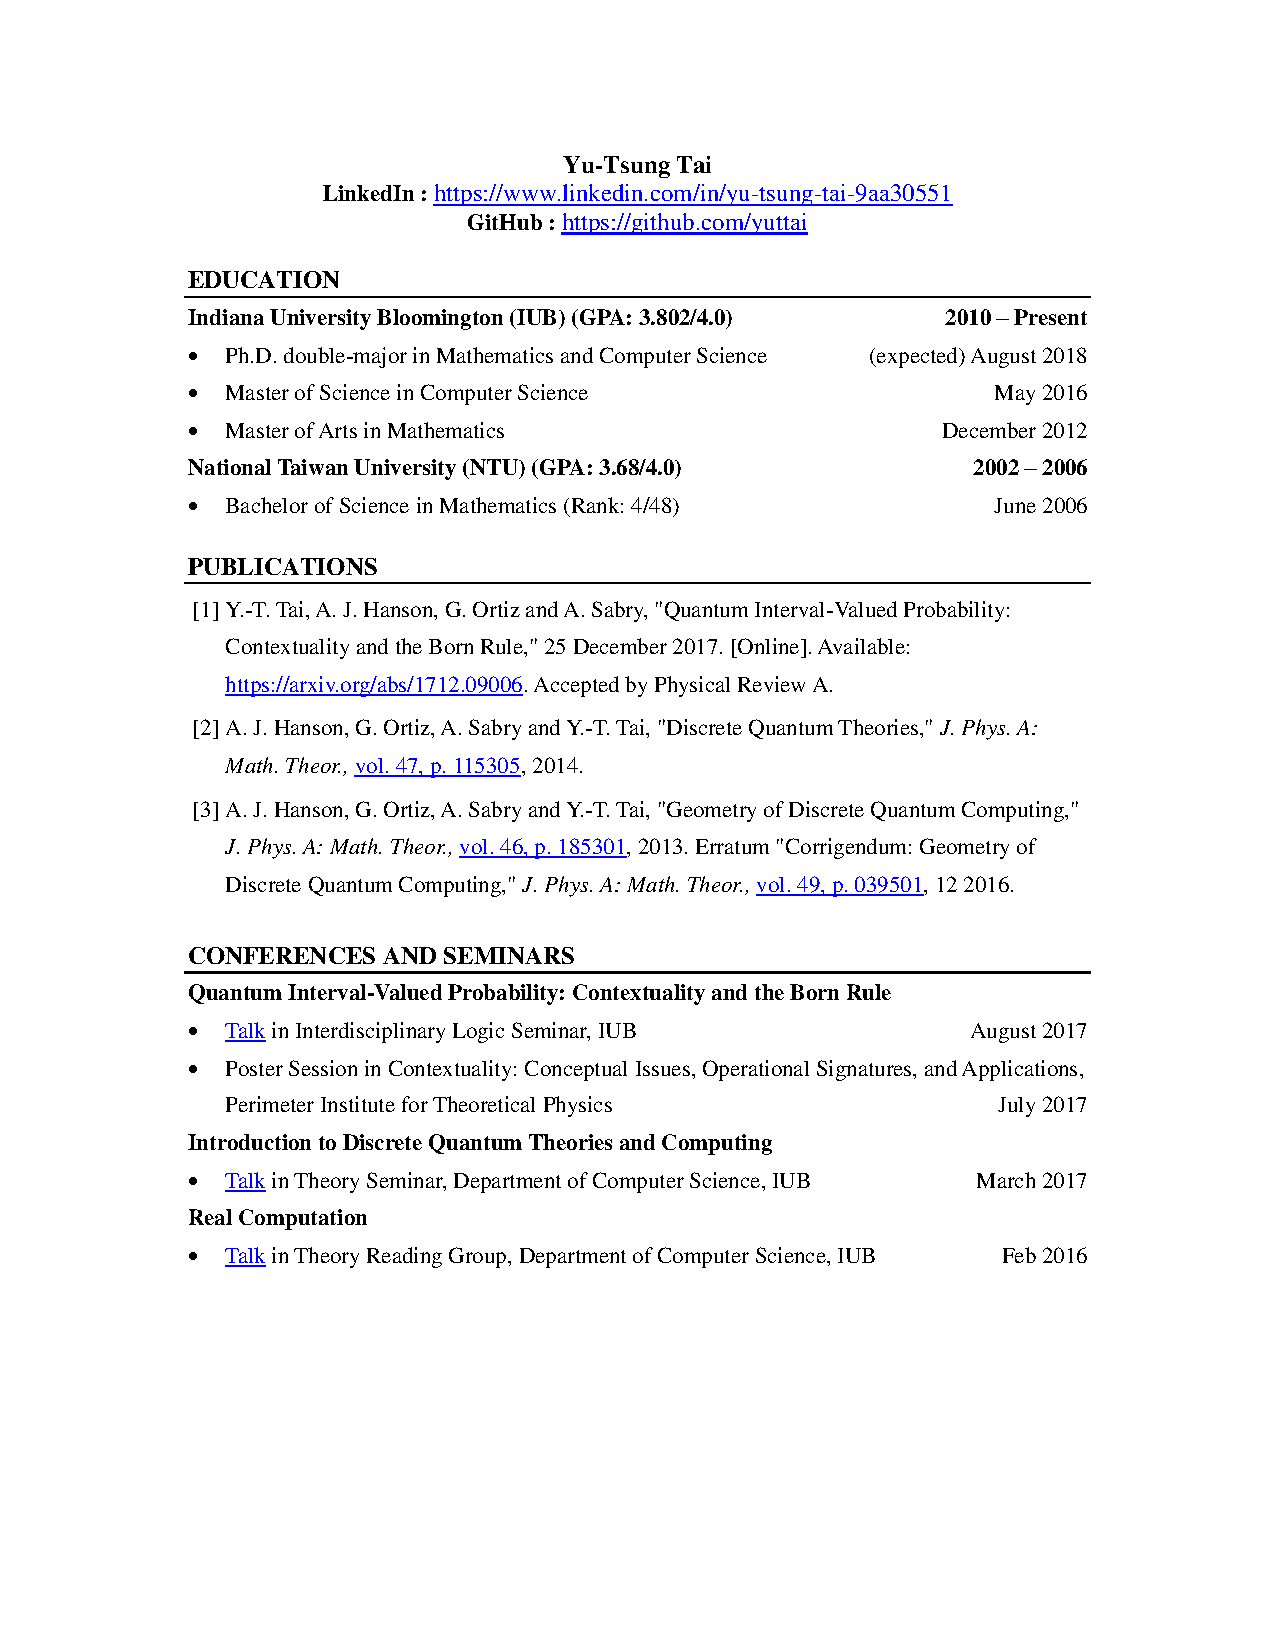
\includepdf[pages=-]{CV_thesis}
\end{document}